\documentclass[10pt]{article}
\usepackage[T1]{fontenc}
\usepackage{lmodern}
\usepackage[margin=1in]{geometry}
\usepackage{graphicx}
\usepackage{booktabs}
\usepackage[numbers,sort&compress]{natbib}
\usepackage[hidelinks]{hyperref}

\newcommand{\code}[1]{\texttt{#1}}
\newcommand{\ci}[3]{$#1$ [$#2$, $#3$]}
\setlength{\tabcolsep}{5pt}
\setlength{\emergencystretch}{1.5em}
\setlength{\bibsep}{1pt plus 1pt}
\renewcommand{\bibfont}{\footnotesize}
\setlength{\textfloatsep}{10pt plus 2pt minus 2pt}
\setlength{\floatsep}{8pt plus 2pt minus 2pt}
\setlength{\intextsep}{8pt plus 2pt minus 2pt}
\setlength{\abovecaptionskip}{3pt}
\setlength{\belowcaptionskip}{2pt}
\renewcommand{\topfraction}{0.9}
\renewcommand{\bottomfraction}{0.8}
\renewcommand{\textfraction}{0.1}
\renewcommand{\floatpagefraction}{0.8}
\makeatletter
\renewcommand\paragraph{\@startsection{paragraph}{4}{\z@}{1ex plus .3ex minus .2ex}{-1em}{\normalfont\normalsize\bfseries}}
\renewcommand\section{\@startsection{section}{1}{\z@}{2ex plus .5ex minus .2ex}{0.8ex plus .2ex}{\normalfont\large\bfseries}}
\makeatother

\title{Because: preregistered randomized tests of what makes a coding agent follow its instructions}
\author{Abhay Mettu}
\date{November 2026. Preprint, not peer reviewed.}

\begin{document}
\maketitle

\begin{abstract}
\noindent People write instruction files for coding agents on folk beliefs: give a reason, write MUST, put the important rule first, phrase a skill's description as a list of triggers. We tested these on Claude Code 2.1.303 with Sonnet 5.5 at medium effort in three preregistered randomized studies, with outcomes decided by code. Study 1 (1,000 runs, 7,072 observations on nine rules) crossed reason clauses with wording features. Its registered reading is inconclusive. The bar for calling a reason null was an upper bound under 5 points, and the real reason reached 5.7 ($+0.2$, 95\% CI $-5.2$ to $+5.7$). The data exclude effects above about 6 points for a real reason on rules like these. A placebo reason is $+1.1$ ($-1.2$ to $+3.5$), real and placebo are equivalent within 5 points (TOST $p = .040$), the Langer analogue does not reproduce, and no wording factor survives Holm. Study 2 (598 runs) finds that a trigger-list description beats one short sentence while the description is in view ($+17.6$ points) and that an early name beats a late one at 300 skills ($+51.3$). We measured the CLI's listing rule with no model judgment. Study 2b (534 runs) finds that past the listing budget a short description beats a long trigger list by 29.8 points, and that a short description in trigger form beats it by 29.4 while costing under 10 points below the budget ($+2.1$, $-2.5$ to $+6.7$).
\end{abstract}

\section{The question}

This paper tests whether the wording of an instruction file changes what a coding agent does. Files such as \code{CLAUDE.md} and \code{AGENTS.md} are where a repository tells an agent how to work, and the people who write them follow folk rules: give a reason, write MUST, put the important rule first, keep the file short, write a skill's description as a list of triggers or as ``ALWAYS invoke''. A census of public repositories finds a median instruction set of 818 words, finds that 74.0\% of directives give no reason, and says of the causal question, ``Whether reasons or emphasis change what agents do remains open'' \citep{zarzycki2026}.

The folk rules matter because they decide where effort goes. If a reason clause raises compliance, a team should explain every rule to the agent. If it does not, that writing buys nothing the agent acts on, and the effort belongs elsewhere. Skills add a second problem, since a well-written description does nothing if the CLI drops it from the listing before the model sees it.

We ask three questions. Does a reason clause raise compliance, and does a reason with no content work as well as a real one? How much does each folk wording feature move compliance on the same rules? When does a skill's description decide whether the skill loads? We answer them with three registered studies, frozen at the git tags \code{prereg-study1}, \code{prereg-study2} and \code{prereg-study2b}. Section~\ref{sec:deviations} lists every deviation, including one rewrite of the git history. All claims are about Claude Code 2.1.303 and Sonnet 5.5 at medium effort, on these rules and tasks. We make no claim about other agents, models or CLI versions, about what a reason does for a person reading the file, or about how a model processes a reason.

\section{Related work}

\paragraph{Instruction-file censuses and audits.} \citet{zarzycki2026} counts what files say and makes no causal claim. \citet{wang2026evolution} find that a rule raises the rate at which an agent takes a required action by $+0.23$ on average across four agents, and that on four open models a prose-only revision moves compliance by $+0.017$, inside an equivalence margin of 0.08. \citet{zhang2026guardrails} report that random rules match curated ones (both 63.8\%). \citet{zhu2026precedent} find that repository precedent beats an agent's default in 359 of 360 trials, and that a written priority rule succeeds in 59 of 60 trials against 38 of 60 for a code example. \citet{xu2026stale} find that 90.1\% of choices follow a stale file over the code, and one precedence sentence moves code-following from 4.2\% to 91.4\%. None of these randomizes a reason.

The closest work is \citet{mcmillan2026}, who ran 1,650 Claude Code sessions varying file size from 25 to 500 lines, position, architecture and conflict, on one trivial rule always justified as an audit requirement. All four came out null after correction, and its intervals rule out effects above about 6 points on position and architecture. A gap of 26.2 points between two tasks exceeded every structural effect. Reason was held constant there. Position and length in our Study 1 are registered replications of that work.

\paragraph{Skill loading.} \citet{liu2026routing} own the library-size result: with 1,000 irrelevant skills, loaded-skill recall falls from 73.6\% to 27.4\%, and masking distractor descriptions restores it to 63.3\%. They never vary the target's own description. In a preregistered study of two OpenAI models, \citet{wang2026advertising} find that praise in a tool description raises its pick rate by about 43 points. \citet{spence2026} runs about 250 sandboxed Claude Code calls and reports activation of about 100\% for prompts with a keyword, 20\% to 40\% for generic phrasing and about 0\% for indirect phrasing, testing hooks and not description wording. \citet{zhang2026estimands} shows that conditioning on a trigger inside the treated run does not identify an invocation effect, which is why we count loads at any point in a run and score intention to treat.

\paragraph{Prompt emphasis.} \citet{zhan2026wording} show that wordings a verifier treats as equal shift compliance in chat replies: 54.9\% for the positive form, 48.2\% for a longer one, 36.7\% with the target later and 33.8\% for AVOID. They have no reason factor and no instruction file. \citet{lauziere2026} fit regressions on crossed prompt components, the nearest factorial method, on two open models. One informal practitioner test, sample unverified, reports that a consequences strategy did not improve adherence \citep{inferal}.

\paragraph{The Langer line and its critics.} Our analogy comes from Experiment 1 of \citet{langer1978}, 120 adults at a copier. For a 5-page favor, compliance was .60 with no information, .93 with a placebic reason (``because I have to make copies'') and .94 with a sufficient one. For a 20-page favor it was .24, .24 and .42. The small-favor result rests on about 15 people per cell. \citet{folkes1985} reports of two further studies that ``Neither study replicated Langer et al.'s results.'' We treat this as an analogy to a contested paradigm and not as a replication target.

\paragraph{What is new and what is not.} To our knowledge, no preregistered randomized test of a reason or a placebo reason on a real coding agent has been published. That statement rests on about 29 searches before the freeze and a shorter repeat on 2 November 2026. Practitioner tests exist and this field moves weekly, so a missing hit is not proof. Position and length replicate \citet{mcmillan2026}, and library size belongs to \citet{liu2026routing}. Our contribution is the combination: reason, placebo, modal, emphasis and example crossed over nine rules on one real agent, and the target skill's own description randomized on real Claude Code, crossed with library size.

\section{Study 1: design}\label{sec:design1}

\paragraph{Why focal rules.} Compliance sits at the ceiling for most rules, and wording cannot move a rule already followed. Of 59 candidates (\code{docs/POOL.md}), 41 were dropped at the ceiling in pilots, and that share is itself a finding. The pool rule required shown compliance within 0.10 to 0.95 and no-rule compliance at or below 0.50, computed on compliance pooled across arms and never on a contrast. The manual steps, taken without reference to arms, were these: \code{line\_length} dropped as a weaker form of \code{line\_60}; \code{short\_final} dropped because a short message passes three other rules mechanically; \code{one\_blank} and \code{no\_chain} reworded so that the rule says what the checker measures. Nine focal rules remained (Table~\ref{tab:rules}). All claims are about them, which means rules an agent lapses on and not rules in general. Five more stay in the files as ballast and are reported descriptively only.

\paragraph{Split-plot randomization.} Each run is one \code{claude -p} on one task. Its \code{CLAUDE.md} holds 11 of the 14 rules, shuffled among inert filler rules, and every shown rule's wording is drawn independently and uniformly (Table~\ref{tab:factors}). Rules and tasks are fully crossed over 2 synthetic Python repositories with 3 tasks each. The assignment is committed row by row in \code{data/study1/manifest.jsonl}, with the seed derived from the study name. The batch aborts on any Claude Code version other than 2.1.303 or any model other than \code{claude-sonnet-5-5}. Runs have six tools, at most 40 turns and a 600 s timeout. Claude Code's own preamble (``IMPORTANT: ... you MUST follow them'') wraps the file in every run, confirmed from captured requests, so every emphasis effect here is marginal to it.

\begin{table}[t]\centering\small
\caption{Factors of Study 1. Census 10th and 90th percentiles of file length are about 160 and 3,010 words \citep{zarzycki2026}.}\label{tab:factors}
\begin{tabular}{lp{4.75in}l}\toprule
Factor & Levels & Set per\\\midrule
REASON & none; filler; placebo; norm; real (Table~\ref{tab:clauses}) & rule\\
MODAL & plain imperative; ``You must'' & rule\\
PREFIX & none; \code{IMPORTANT:} & rule\\
CASE & normal; operative word in capitals & rule\\
EXAMPLE & absent; present (``For example: break a long call after its opening bracket.'') & rule\\
POSITION & from the shuffle; top, middle or bottom third of the file by word count & rule\\
LENGTH & short, mean 514 words (450 to 569); long, mean 3,526 words (3,427 to 3,583) & run\\
PRESSURE & none; a task sentence asking for speed and a minimal change & run\\\bottomrule
\end{tabular}
\end{table}

\paragraph{Why filler is the comparator.} A clause changes a rule's length as well as its meaning, and length alone moved compliance by 6.7 points in \citet{zhan2026wording}, so reason versus no clause confounds the two. The filler arm adds a non-reason sentence of matched length and is the primary comparator. Filler might not be inert, since calling a rule ``one of several notes'' could demote it, so the reading also requires an advantage over no clause. Filler, placebo and norm each have 6 paraphrases, dealt without repeats within a file.

\paragraph{Clause manipulation check.} Eight blind raters (Haiku 5.5, no arm labels) scored each clause out of 5 for specific information and for how strongly it asserts obligation (Table~\ref{tab:clauses}, \code{results/clause\_check.json}). Real clauses carry information and the others do not. An earlier placebo set rated 3.9 on obligation, so it was rewritten before the freeze. Norm carries some obligation, which is why it is a separate arm. The real reasons are invented. No voice assistant or ticket importer exists in the repositories, so this arm tests a specific plausible rationale and not a true one. Each shares no content word with its rule.

\begin{table}[t]\centering\small
\caption{What each REASON arm adds to ``Keep every line of Python you write to 60 characters or fewer'', with mean ratings out of 5.}\label{tab:clauses}
\begin{tabular}{lp{3.85in}cc}\toprule
Arm & Text & Information & Obligation\\\midrule
none & (nothing) & & \\
filler & ``This note is one of several notes kept here in this section.'' & 1.0 & 1.0\\
placebo & ``because that is just how this particular part of the project is'' & 1.0 & 1.8\\
norm & ``because that is how we do things here in this repository'' & 1.0 & 2.9\\
real & ``because the on-call team reads code on phones when something breaks at night'' & 4.9 & 2.2\\\bottomrule
\end{tabular}
\end{table}

\paragraph{Isolation and its proof.} A study of instruction following is void if the agent also sees the operator's own instructions, and every run here uses a login on a working developer machine. The harness excludes the user's instruction file, settings, hooks, memory and MCP servers, empties the environment and the home directory seen by tool calls, and rewrites the login email and OS user in a capture proxy. Pilots found three leaks in captured requests (the email, the git user and the shell profile), all fixed before the freeze. \code{make isolation} proves the setup by sending one prompt twice through the proxy, once isolated and once as a plain \code{claude -p}, and scanning the requests (\code{results/isolation.json}). Lines of the operator's instruction and memory files found: 0 of 231 isolated and 219 of 231 plain. Skill names found: 1 of 85 and 73 of 85, the one being the ordinary word ``research'' in the default system prompt. Tools offered: 6 and 181. The plain column is the negative control. During the study a leak scan reads every request of every run, and a run that trips it is excluded and counted.

\paragraph{Checkers and the blind audit.} Compliance is binary per rule per run, decided by code from the transcript and the final repository (\code{study1/rules.py}). No model judges any outcome. Every checker passes a hand-built compliant trace and fails a hand-built violating one. The primary analysis is intention to treat, so a run that never reached a rule's opportunity counts as not complied. The blind audit ran on the finished batch before any contrast was computed. It drew 100 focal observations stratified by rule and outcome, with arm labels removed and the key kept outside the repository until the audit closed. Three fresh model readers each took a third and judged from the rule text and the trace before opening any checker. They decided no outcome. Their job was to find checker faults.

Of the 100 items, 92 agree with the checker, 7 are unclear with the reader's lean matching the checker, and 1 disagrees. All 8 turn on one question, whether a rule's ``you write'' reaches throwaway code that never lands in the repository. Before any contrast, we decided that no checker changes. A code-form rule scores the code the run leaves in the repository, and the Write tool rule scores the action, including a scratch file. Because one reader read an item the other way, we report a sensitivity with \code{write\_tool} scored on repository paths only: 41 verdicts change, real becomes \ci{+0.0}{-5.3}{+5.3} and placebo \ci{+0.9}{-1.4}{+3.1}, so the reading does not change. With about 20 items per reason arm, the audit can find a checker fault and cannot show a small difference in checker error by arm.

\paragraph{Estimator and tests.} We fit OLS on the probability scale with run fixed effects, rule intercepts and a separate coefficient for each rule and factor level. Each contrast yields one estimate per focal rule. The reported effect is their equal-weighted mean, with a t interval across rules ($df = 8$), which treats rules as sampled stimuli \citep{clark1973,judd2012}. That interval is the claim about new rules like these. A studentized randomization test (2,000 permutations within rule) is the finite-population sensitivity. Run-level factors have no run fixed effects, and their standard error is by-run variance plus across-rule variance beyond its sampling part.

Family 1 is H1 (real versus filler) and H2 (placebo versus filler), two-sided, Holm across the two \citep{holm1979}. H3 asks whether a placebo keeps at least half the real effect, and it runs only if H1 is positive and passes. Real minus placebo is reported in all cases, with a TOST at $\pm 5$ points \citep{schuirmann1987} as a registered sensitivity. Family 2 is nine contrasts under Holm. The positive control restates one unshown rule in the task prompt in about 10\% of runs. The reading is applied by \code{reading()} in the code (Table~\ref{tab:reading}), so nobody applies the table by hand.

\begin{table}[t]\centering\footnotesize
\caption{The registered reading of Study 1. Rows are checked in order, and ``passes'' means Holm-adjusted $p < .05$.}\label{tab:reading}
\begin{tabular}{p{3.0in}p{3.2in}}\toprule
Result & Reading\\\midrule
Positive control under 30 points & Assay failed; nothing is read\\
H1 and H2 pass and are positive, H3 passes, real and placebo each above no clause ($p < .05$) & The form of a reason moves compliance, and if the TOST passes, a placebo does about as much as a real reason\\
H1 passes and is positive, H2 does not, H3 fails, real above placebo ($p < .05$) & Reasons work through their content; a placebo does not substitute\\
H1 and H2 do not pass, both upper CI bounds under 5 points & A reason clause does not move compliance by a practically useful amount on these rules\\
Anything else & Inconclusive, and said so\\\bottomrule
\end{tabular}
\end{table}

\paragraph{Power, registered and realized.} The registration simulated 1,000 runs from pilot rates and called the study well powered for about 8 points and underpowered for 5. Simulating on the real assignment (\code{results/calibration.json}) gives lower figures, shown with the Holm worst case in parentheses. A true 5-point effect has power 0.56 (0.41) against a registered 0.62 (0.49) at slope SD 3, and 0.34 (0.20) against 0.40 (0.26) at slope SD 6. A true 8-point effect has 0.91 (0.81) against 0.94 (0.84), and 0.68 (0.53) against 0.74 (0.59). The registered test's false positive rate at .05 with no planted effect is 0.053 over 1,000 simulations, so it holds its level. The run-level test rejected in 0.000 of those simulations, so it is conservative, and the long and urgent contrasts lose power to that.

\section{Study 1: results}\label{sec:results1}

All 1,000 runs were used, giving 7,072 focal observations and overall focal compliance of 0.579. There were no errors, leaks, timeouts or turn-limit runs, and the repository's tests passed in every run. Observations by reason arm are 1,439 none, 1,449 filler, 1,386 placebo, 1,447 norm and 1,351 real. The positive control cleared its 30-point bar: 0.653 named in the prompt (n 72) against 0.038 with no rule (n 1,856). The assay can detect change.

\begin{table}[t]\centering\small
\caption{Study 1 contrasts in percentage points (\code{results/NUMBERS.md}). Top block: family 1 and the reported reason contrasts, with Holm across H1 and H2 only. The H3 gate stayed closed because H1 did not pass, so its row decides nothing. Bottom block: family 2, Holm across the nine.}\label{tab:family1}
\begin{tabular}{lccc}\toprule
Contrast & Points [95\% CI] & $p$ & Holm $p$\\\midrule
H1 real vs filler & \ci{+0.2}{-5.2}{+5.7} & .924 & .924\\
H2 placebo vs filler & \ci{+1.1}{-1.2}{+3.5} & .300 & .599\\
H3 placebo minus half of real & \ci{+1.0}{-1.5}{+3.6} & .375 & \\
Real minus placebo & \ci{-0.9}{-5.6}{+3.8} & .666 & \\
Real vs no clause & \ci{+1.4}{-3.9}{+6.8} & .549 & \\
Placebo vs no clause & \ci{+2.4}{-1.4}{+6.1} & .189 & \\\midrule
Norm vs filler & \ci{+0.2}{-4.1}{+4.4} & .927 & 1.000\\
No clause vs filler & \ci{-1.2}{-6.7}{+4.2} & .622 & 1.000\\
``You must'' vs plain & \ci{-0.3}{-2.2}{+1.6} & .755 & 1.000\\
\code{IMPORTANT:} vs none & \ci{+1.0}{-2.4}{+4.5} & .507 & 1.000\\
Capitals vs normal & \ci{+2.5}{+0.2}{+4.9} & .039 & .353\\
Example vs absent & \ci{+1.4}{-6.2}{+9.1} & .676 & 1.000\\
Top vs bottom third & \ci{+3.8}{-1.3}{+9.0} & .126 & .884\\
Long vs short file & \ci{-3.7}{-8.2}{+0.7} & .090 & .720\\
Urgent vs no pressure & \ci{-4.3}{-14.1}{+5.5} & .338 & 1.000\\\bottomrule
\end{tabular}
\end{table}

\paragraph{The registered reading is ``inconclusive''.} The code returned that word and we report it as registered (Table~\ref{tab:family1}). The bar for calling a reason null was an upper bound under 5 points, and the real reason reached 5.7. H1 and H2 do not pass, so no positive reading applies, and that bound rules out the null reading.

\paragraph{What the data does support.} Effects above about 6 points are excluded for a real reason on rules like these. A placebo is \ci{+1.1}{-1.2}{+3.5}. Real and placebo are equivalent within 5 points (TOST $p = .040$). That TOST is a registered sensitivity, and because ceilings shrink realized gaps it passed in 20.0\% of pre-freeze simulations with a nominal real effect of 5 and a placebo of 0 (\code{docs/REVIEW-2-prereg.md}). The Langer analogue does not reproduce here. In that paradigm a placebic reason does what a real one does and the favor's size decides whether either works. Here neither moved compliance detectably, and the moderator of reason by pressure, a loose analogue of the favor split, shows nothing (secondary, no significance claim): real \ci{-0.1}{-5.0}{+4.8}, placebo \ci{-1.3}{-5.3}{+2.6}, norm \ci{+0.4}{-7.5}{+8.2}. The randomization test agrees, at $p = .917$ for real and $p = .300$ for placebo. Rule by rule, the real reason runs from $-8.1$ points on \code{func\_lines} to $+15.8$ on \code{final\_no\_first\_person} (\code{results/study1.json}), and nine rules cannot say whether that spread is signal.

\paragraph{Wording.} No wording factor survives Holm (Table~\ref{tab:family1}, Figure~\ref{fig:s1}). Capitals come closest, with an unadjusted $p$ of .039 and an adjusted $p$ of .353. ``You must'' has the tightest interval, $-2.2$ to $+1.6$ points. Position and length are registered replications of \citet{mcmillan2026}. Neither differs detectably, though their intervals hold effects of several points. The registered sensitivity for run-level factors, shown minus unshown, gives long versus short \ci{-2.7}{-8.0}{+2.7} and urgent versus none \ci{-2.7}{-13.9}{+8.5}.

\begin{figure}[t]\centering
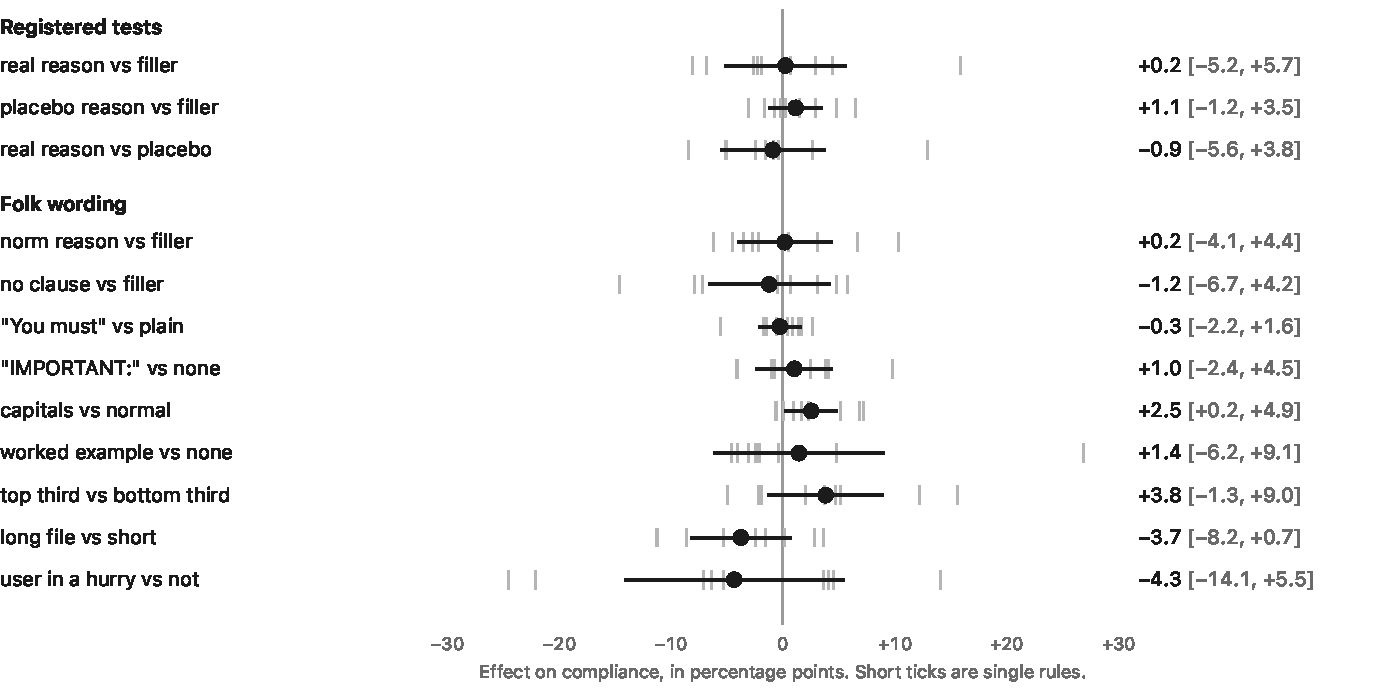
\includegraphics[width=0.78\linewidth]{figures/study1-effects.pdf}
\caption{Study 1 effects with 95\% intervals. Each short tick is one rule.}\label{fig:s1}
\end{figure}

\section{Study 2 and the measured listing mechanism}\label{sec:study2}

\paragraph{The listing rule.} Claude Code tells the model which skills exist through a listing whose descriptions share a character budget. We measured how the CLI fills it (\code{docs/LISTING-MECHANISM.md}). If every entry fits in the budget, which is 30,000 characters on Sonnet 5.5 and Haiku 5.5, read to within 3, every skill keeps its description. Otherwise bundled skills keep theirs, every other skill is charged for its bare name, and the rest are sorted by usage score with ties in name order. The CLI walks that list once. A skill keeps its description if it fits what is left, and if it does not fit the walk continues, so a short description further down can still fit. Usage score is $\mathit{usageCount} \times \max(0.5^{d/7}, 0.1)$, with $d$ the days since last use, so one call outranks every never-used skill.

This rule is a property of Claude Code 2.1.303. It was measured with no model judgment, by comparing the entries that carry descriptions in the requests the CLI sent against what the rule predicts. Over 4,915 listing entries it made 0 errors. Removing usage from the rule gives 28 errors on the 2,590 entries of the pilot captures. Eight variants gave the identical described set and order, which rules out relevance to the prompt, the tool list, model and context size among these models, creation order, modification time and nondeterminism. An older model differs through the budget: \code{claude-sonnet-4-6} reads below 10,240. In a sample from a public library the budget binds between 100 and 150 skills (\code{results/listing\_budget.json}). The decay term was read from the code in the shipped CLI and not tested live.

\paragraph{Design.} Each run has one of 12 target skills, with a fixed body and one of 5 description wordings: minimal (``Reconciles ledgers.''), padded (minimal plus a content-free sentence matching a trigger list's length), trigger (``Use when ...''), trigger\_not (trigger plus ``Not for ...'') and directive (``ALWAYS invoke this skill when ... You MUST use it ...''). Library is 0, 50 or 300 distractors, at 25\%, 25\% and 50\% of runs, sampled from 388 real skills of a public MIT-licensed library. Name prefix is \code{aa-} or \code{zz-}, an artificial stand-in for early and late. Prompts are keyword, generic, indirect or decoy, the last being a nearby request that does not need the skill. Each run's target has a unique name, so none starts with usage, though distractors invoked in one run do gain rank later. Version, model, effort and isolation are as in Study 1, with the Skill tool added and a limit of 6 turns. A load is a Skill call naming the target or a Read of its \code{SKILL.md} at any point in the run, decided by code. Contrasts are per target and averaged with equal weight, with a t interval across targets and Holm across the family.

\paragraph{Results.} Of 600 planned runs, 598 were used. Two were excluded by the leak scan on the needle \code{agent-memory/}, which matches a public distractor's text. Load rates by prompt were 0.877 keyword, 0.660 generic, 0.752 indirect and 0.007 decoy.

\begin{table}[t]\centering\small
\caption{Study 2 family, Holm across the five, in percentage points (\code{results/NUMBERS.md}). The $+0.0$ rows are ties at a bound, and their zero-width intervals are not evidence of no effect.}\label{tab:study2}
\begin{tabular}{lccc}\toprule
Contrast & Points [95\% CI] & $p$ & Holm $p$\\\midrule
C1 trigger vs minimal, in view & \ci{+17.6}{+6.3}{+29.0} & .006 & .023\\
C2 directive vs trigger, in view & \ci{+0.0}{+0.0}{+0.0} & 1.000 & 1.000\\
C3 ``Not for'' clause, false loads, in view & \ci{+0.0}{+0.0}{+0.0} & 1.000 & 1.000\\
C4 \code{aa-} vs \code{zz-} at 300 skills & \ci{+51.3}{+37.7}{+64.8} & $<.001$ & $<.001$\\
C5 trigger vs minimal, 300 skills, \code{zz-} & \ci{-27.1}{-67.1}{+13.0} & .154 & .462\\\bottomrule
\end{tabular}
\end{table}

C1 is real (Table~\ref{tab:study2}). With the description in view a trigger list loaded the skill in 65 of 65 non-decoy runs and one short sentence in 56 of 68 (\code{paper/counts.json}), an estimate of $+17.6$ points that survives Holm. Length alone does not explain it, since padded versus minimal is \ci{-6.7}{-23.2}{+9.8} as a secondary.

C2 and C3 sat at a ceiling and a floor. Directive loaded in 72 of 72 runs and trigger in 65 of 65. On decoy prompts the ``Not for'' wording falsely loaded in 0 of 18 runs and trigger in 0 of 24. When every target ties, the spread across targets is zero, so the t interval degenerates to a point and the reported $p$ of 1.000 comes from a rule for ties in the code (Section~\ref{sec:deviations}). These zeros are not evidence of no effect. The design left no room to see one. Across all 138 decoy runs there was one false load, on a minimal description in a library of 0.

C4 is $+51.3$ points. C5 was too wide. Only 8 of 12 targets were estimable, and the interval of $-67.1$ to $+13.0$ cannot separate the wordings. The point estimate leaned toward reversal: at 300 skills with a late name minimal loaded at 0.61, trigger at 0.24 and directive at 0.36, and only minimal ever kept its description (0.65 of runs against 0.00). Study 2b was registered to settle this. C5 also lets wording change whether the description is present, since a short one can fit the leftover budget. As a secondary with no correction, library 300 versus 0 with an \code{aa-} name is \ci{-10.3}{-18.0}{-2.5}.

\section{Study 2b: the reversal past the budget}\label{sec:study2b}

\paragraph{Design.} We wrote this study after reading Study 2, and none of its data was seen when its hypotheses were set. All names are \code{zz-} and none repeats a Study 2 target. It adds one wording, short\_trigger, a mechanical rewrite of the minimal text into trigger form (``Use when reconciling ledgers.''). Mean lengths are 21 characters for minimal, 32 for short\_trigger and 140 for trigger. The 12 targets are crossed with the 3 wordings, at 12 runs per cell at 300 distractors and 4 at 50, for 576 planned. Decoys are dropped. Three distractors invoked in Study 2 keep their rank, the same across arms. Power to detect 30 points at the worst case of Holm over four tests is 0.76 to 0.94, and for 20 points 0.37 to 0.60, both assuming a spread of 10 to 20 points between targets.

\paragraph{Results.} We used 534 runs. Another 41 were not run, because the registered six-point quota counter read the whole account while Study 1 ran at the same time, which the registration did not anticipate. The batch stopped at 535 of 576, and the registration says whatever exists is analyzed. One further run is excluded by the leak scan, a false positive on the needle \code{agent-memory/}, which appears in a public skill's text.

\begin{table}[t]\centering\small
\caption{Study 2b family, Holm across the four, in percentage points.}\label{tab:study2b}
\begin{tabular}{lccc}\toprule
Contrast & Points [95\% CI] & $p$ & Holm $p$\\\midrule
D1 minimal vs trigger, 300 skills & \ci{+29.8}{+19.2}{+40.3} & $<.001$ & $<.001$\\
D2 short\_trigger vs trigger, 300 skills & \ci{+29.4}{+20.5}{+38.4} & $<.001$ & $<.001$\\
D3 short\_trigger vs minimal, 300 skills & \ci{-0.3}{-9.2}{+8.6} & .939 & .939\\
D4 short\_trigger vs trigger, 50 skills & \ci{+2.1}{-2.5}{+6.7} & .339 & .678\\\bottomrule
\end{tabular}
\end{table}

Both registered readings fired (Table~\ref{tab:study2b}). The code returned, ``past the budget a short plain description beats a long trigger list; a short description that says when to use the skill beats a long one past the budget and costs under 10 points below it.'' D1 replicates the direction of C5 with a usable interval. D4's lower bound of $-2.5$ clears the registered floor of $-10$. D3 shows no difference between the two short wordings at 300 skills. Table~\ref{tab:grid} gives the cells, and Figure~\ref{fig:reversal} shows the crossing in both studies. The trigger wording never kept its description at 300 skills here, and it still loaded in 0.211 of runs, from the name alone.

\begin{table}[t]\centering\small
\caption{Study 2b by library and wording. ``Reached model'' is the share of runs whose request held the target's description. The last two columns are exploratory, because whether a description fits depends on the distractors a run drew and is not randomized.}\label{tab:grid}
\begin{tabular}{llccccc}\toprule
Library & Wording & Load rate & n & Reached model & Load if reached & Load if not\\\midrule
50 & minimal & 0.953 & 43 & 1.000 & 0.953 & \\
50 & short\_trigger & 1.000 & 44 & 1.000 & 1.000 & \\
50 & trigger & 0.978 & 46 & 1.000 & 0.978 & \\
300 & minimal & 0.511 & 137 & 0.526 & 0.750 & 0.246\\
300 & short\_trigger & 0.500 & 136 & 0.338 & 0.848 & 0.322\\
300 & trigger & 0.211 & 128 & 0.000 & & 0.211\\\bottomrule
\end{tabular}
\end{table}

\begin{figure}[t]\centering
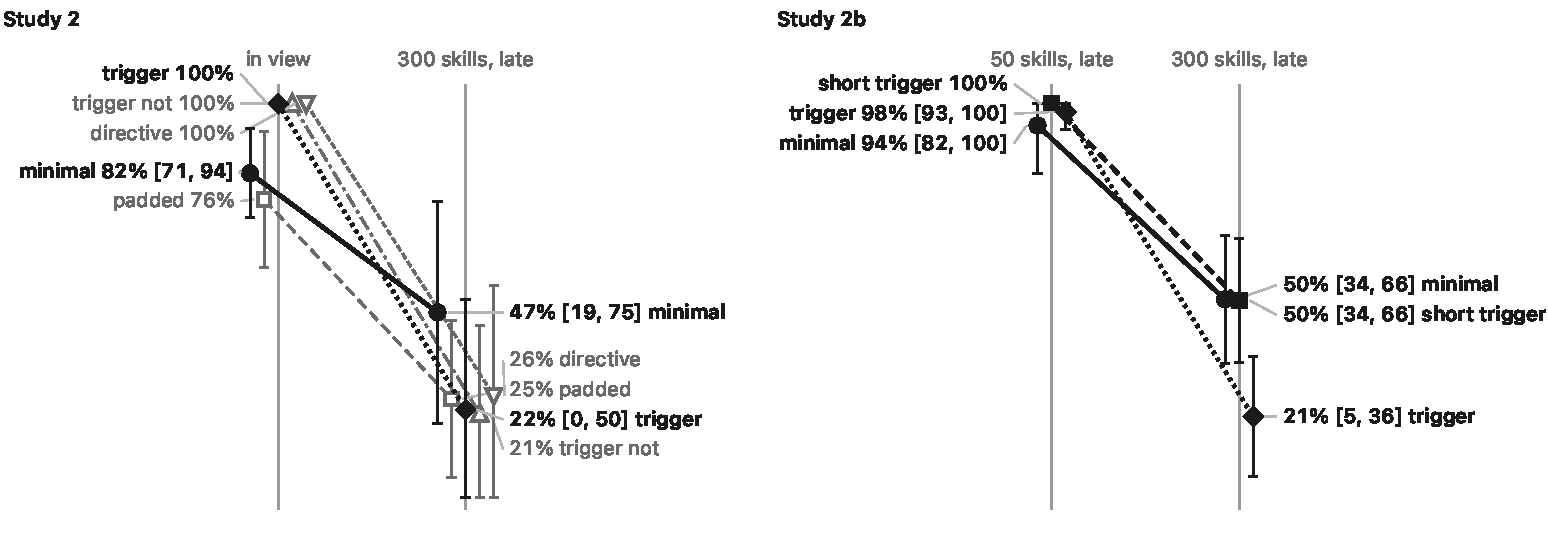
\includegraphics[width=0.94\linewidth]{figures/reversal.pdf}
\caption{Load rate by wording. Left, Study 2 (in view pooled over the visible cells, non-decoy runs). Right, Study 2b. Trigger lists lead in view and fall below the short wordings once the budget binds.}\label{fig:reversal}
\end{figure}

\section{Exploratory results}\label{sec:exploratory}

None of this section is a registered test. Its numbers come from \code{results/exploratory.json} and \code{results/robust.txt}.

\paragraph{Which rule it is.} Focal compliance runs from 0.09 to 0.93 by rule, with an SD of 0.29 (Table~\ref{tab:rules}). The pool rule admitted rules between 0.10 and 0.95 in pilots, so selection set this range by construction, and it is not an estimate over rules in general. Leaving one rule out moves H1 between $-2.2$ and $+1.3$ points. The ballast rules, not analyzed, sat at 0.94 to 0.99.

\paragraph{Having a rule, and restating it.} Shown minus no rule is \ci{+54.2}{+33.1}{+75.2} points. The no-rule baseline is not a clean ``no instruction'' state, because other rules are present. Named in the prompt minus shown in the file is \ci{+7.1}{+0.2}{+13.9} points, higher on 8 of 9 rules. This rests on 3 to 11 runs per rule, so it is a lead for a registered test and nothing firmer.

\begin{table}[t]\centering\footnotesize\setlength{\tabcolsep}{3pt}
\caption{Focal rules and compliance by rule, across all wordings. Named in the prompt rests on 3 to 11 runs per rule.}\label{tab:rules}
\begin{tabular}{lcccc}\toprule
Rule (bare wording) & Shown & No rule & Named & n shown\\\midrule
Do not use contractions or apostrophes in your final message. & 0.87 & 0.28 & 1.00 & 786\\
Do not use digits in your final message; spell numbers out. & 0.09 & 0.00 & 0.14 & 786\\
Do not use the words I, my, we or our in your final message. & 0.32 & 0.00 & 0.38 & 786\\
Keep every Python function you write, including its signature, to 8 lines or fewer. & 0.44 & 0.00 & 0.30 & 786\\
Keep every line of Python you write to 60 characters or fewer. & 0.81 & 0.00 & 1.00 & 785\\
Give every variable, parameter and loop variable you write a name of at least 4 letters. & 0.50 & 0.04 & 0.62 & 786\\
Do not leave two blank lines in a row in any Python you write. & 0.41 & 0.00 & 0.50 & 786\\
Sort the import lines of every new Python file in reverse alphabetical order. & 0.84 & 0.00 & 0.91 & 786\\
Create new Python files with your Write tool, not through shell redirection. & 0.93 & 0.00 & 1.00 & 785\\\bottomrule
\end{tabular}
\end{table}

\paragraph{The mixed model.} The registered robustness model (\code{analysis/robust.R}) decides nothing. It gives prediction intervals for a new rule of $-5.7$ to $+5.1$ points for real and $-1.6$ to $+4.4$ for placebo. It has rule slopes only on real and placebo, so its t values for short files (3.93) and urgency ($-4.23$) ignore rule-to-rule variation and are not claims about new rules. The registered estimator allows for it, and those two contrasts do not pass there.

\paragraph{Where calls go past the budget.} At 300 skills in Study 2b, with the target's description gone, the shares are 0.254 target loaded, 0.025 other skill only and 0.721 no skill (n 283). With the description kept they are 0.788, 0.034 and 0.178 (n 118). Study 2 shows the same shape, at 0.29, 0.05 and 0.66 (n 100) against 0.844, 0.000 and 0.156 (n 135). Losing the description goes with using no skill and not with using a wrong one. Fit is not randomized within a wording.

% HAIKUREPLICATION: fill in the sign-only reading of data/study1haiku here, then remove this comment and the visible stub below.
\paragraph{Replication on Haiku.} HAIKUREPLICATION: [to be filled in. Registered as 300 runs of the same design on \code{claude-haiku-5-5}, read for sign only, with no significance claim, on a pool selected on Sonnet.]

\section{Deviations and disclosures}\label{sec:deviations}

All of these are logged in \code{docs/DEVIATIONS.md} with date and reason. The registered analysis is still what is reported.

\paragraph{Both studies.} A bug in the frozen analysis was found on first reading Study 2's output and fixed. \code{by\_rule} returned a NaN $p$ when every rule or target agreed exactly, and the NaN corrupted Holm for the rest of the family, so C4 at $+51$ points first showed an adjusted $p$ of 1.000. A zero standard error now gives $p = 1$ for a zero estimate and $p = 0$ otherwise. It changes results only where such a tie exists.

We rewrote the git history once, on 2 November 2026 and before any public release of the repository, to remove account identifiers. Claude Code tags each request with an account id and a device id, and the sample captures kept them. \code{git filter-repo} removed that one \code{metadata} field from every kept capture in every commit, so the commit and tag hashes changed. Dates, messages and every other file are as they were, and the preregistration files hash to the same git blobs at the new tags as at the old ones (\code{PREREG.md} 2f7f2ff909, \code{PREREG-STUDY2.md} e6002afada, \code{PREREG-STUDY2B.md} 4290c9823c). The order of events rests on the commit dates and the push history of a repository created at the Study 1 freeze, which a reader cannot fully verify from outside. No timestamping service was used.

\paragraph{Study 1.} (1) \code{git add -A} at the Study 2 tag committed about 154 partial Study 1 runs. Nobody had read a contrast, and the final data commit supersedes them. (2) The audit sampler as frozen drew from every shown rule, so it was changed to draw 100 focal observations as registered, and it also gives the reader a diff, because many rules apply only to added lines. (3) With about 260 runs in and before any contrast, an early blind audit of 36 extra observations with no arm labels agreed with 34 and found one fault. \code{write\_tool} failed a run for \code{cat >>} onto a file the repository already had, which the rule does not cover. The checker now ignores a redirect onto a file that existed at the base commit, and all runs were rescored. (4) Harness edits after the tag touch no run's behavior: the leak needle \code{agent-memory} became \code{agent-memory/}, \code{run\_agent} gained a \code{probe} parameter, helpers were factored out, kept samples drop \code{metadata}, and the wrapper shell is written once. The batch ran the code as frozen plus the first two. (5) After the registered audit and before any contrast, the scope of ``you write'' was written down as in Section~\ref{sec:design1}, with no checker changed. (6) The mixed model's export was restricted to focal rules.

\paragraph{Study 2b.} The batch stopped at 535 of 576 on its registered quota stop (Section~\ref{sec:study2b}).

\paragraph{Registered secondaries with no number.} The Study 2 registration asks for C1 minus C5 with its interval and for prompt type by wording, and the Study 2b registration asks for its contrasts within each prompt type. The frozen analyses do not compute these, the result files do not hold them, and we do not report them.

\paragraph{Disclosures from the pre-freeze review (\code{docs/REVIEW-2-prereg.md}).} PRESSURE is an instruction as well as pressure, since ``keep it minimal and skip anything not strictly needed'' can shorten code with no rule in play, and favor size in Langer maps to rule cost more than to user urgency. LENGTH changes target density as well as length. Rules interact mechanically: wrapping for \code{line\_60} adds lines against \code{func\_lines}, and long names from \code{name\_length} do too. Independent labels keep the own-rule contrast unbiased, but a clause on one rule may spill onto another. Final messages sometimes report on other rules, which adds noise and not bias. EXAMPLE adds specification as well as form and has no length-matched control. In the fielded files 60\% of shown rules carry ``because'' against a census rate of 26\%, so a single clause may be diluted relative to a file where it stands out. For prohibitions the proposed ``comply and task complete'' outcome was not implemented. Rules near the top of the band leave little room, and selection brings some regression to the mean.

\section{Limits}\label{sec:limits}

\paragraph{Scope.} Claims read ``Claude Code 2.1.303, Sonnet 5.5 at medium effort, on these rules and tasks''. We ran one model, one CLI version, nine rules and two synthetic repositories for Study 1, and 12 targets written by us for Studies 2 and 2b. The tool list is shorter than the default, which changes the system prompt from what an interactive user sees. Study 1 logged six system prompt hashes, one per task. Wording effects vary by model in the panel of \citet{zhan2026wording}, so a null here may be specific to this model.

\paragraph{Nine rules is few.} The by-rule interval speaks to new rules like these, drawn from the same kind of pool, and with $df = 8$ it rests on a small sample of stimuli. Realized power for a true 5-point effect is 0.34 to 0.56, so a real effect of that size could easily read as this study read.

\paragraph{What a reader should not conclude.} Do not conclude that reasons never matter. The interval allows up to 5.7 points, and rules in conflict with repository precedent were not tested. Do not conclude that reasons are useless in a file, since people read these files too and we measured only the agent. Do not conclude that emphasis has no effect in general, since Claude Code's preamble already supplies IMPORTANT and MUST in every run. Do not read the placebo result as a statement about mindlessness. Do not read the zero rows of Study 2 as showing that ``ALWAYS invoke'' or a ``Not for'' clause does nothing, since both arms sat at a bound. Do not read Study 2b as saying short descriptions are always better. Below the budget the data shows no measurable cost and no gain, and past it the result depends on a CLI rule that another version can change.

\paragraph{Skills.} The \code{aa-} and \code{zz-} prefixes are artificial. A target's name stays informative with no description, so a load past the budget can come from the name alone. Distractors come from one public library. short\_trigger is a mechanical rewrite, and a person writing one by hand might do better. Every target started with no usage history, and by the listing rule one earlier call would change its standing, so nothing here describes a skill already in use. Only project skills and built-ins load here, because the harness passes project settings only. Small synthetic repositories may also read as tests, and thinking text is empty in the raw logs, so demand effects cannot be audited there.

\section{Replication package}

Code, data and the three frozen registrations are in the repository at \url{https://github.com/abhaymettu/because}, under an MIT license. Each confirmatory batch has its manifest, traces, raw streams and sample request bodies under \code{data/}. Study numbers come from \code{results/NUMBERS.md}, which is generated from the results, or from the result file named beside them. From the repository root, \code{git tag -l 'prereg-*'} lists the freezes. \code{make test} and \code{make replay} need no subscription, and \code{make reproduce} regenerates every number from the traces. \code{make isolation} needs a login. \code{python -m analysis.listing\_mechanism replay} checks the listing rule against stored captures, and \code{python -m paper.counts} regenerates the Study 2 cell counts. \code{make rerun} repeats the runs, which needs Claude Code 2.1.303 and a subscription. At API-equivalent prices Study 1 cost \$102.84 (mean 9.3 turns, 33.5 s per run), Study 2 cost \$26.97 and Study 2b cost \$29.52.

\bibliographystyle{plainnat}
\bibliography{refs}

\end{document}
